
 \section{Übertrager}
 \textit{Dieses Kapitel wurde aus dem PVK Skript von Gian Marti übernommen  }

\subsection{Gegeninduktion}
\begin{figure}[H]
\center
\vspace{-0.5cm}
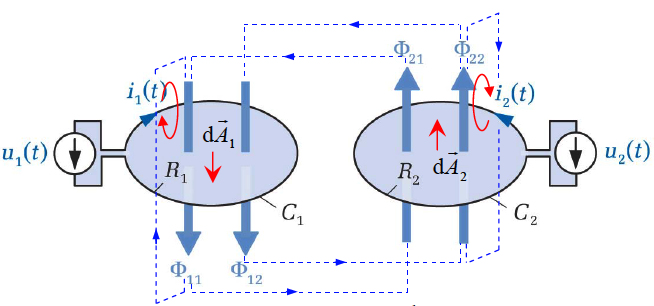
\includegraphics[width=0.65\textwidth]{img/Tra1}
\vspace{-0.2cm}
\end{figure}
Zwei Leiterschleifen werden von zeitlich abhängigen Strömen $i_1(t), i_2(t)$ durchflossen (angeregt durch die Spannungen $u_1(t),u_2(t)$). Dabei erzeugen sie Flüsse $\Phi_{11}, \Phi_{22}$ in ihren jeweiligen Schleifen, aber auch Flüsse durch die jeweils gegenüberliegende Schleife, $\Phi_{12},\Phi_{21}$.
Nun kann man die Selbst- und Gegeninduktivitäten $L_{11},L_{22},L_{12},L_{21}$ defnieren als
$$L_{11} = \frac{\Phi_{11}}{i_1}, \qquad L_{22} = \frac{\Phi_{22}}{i_2}, \qquad L_{12} = \frac{\Phi_{12}}{i_2}, \qquad L_{21} = \frac{\Phi_{21}}{i_1}$$
dann gilt nach dem Induktionsgesetz (das Argument der Zeit, $t$, wird jeweils nicht ausgeschrieben):
\begin{equation*}
\begin{alignedat}{2}
u_1 &= R_1i_1 + \frac{d}{dt}\big(\Phi_{11}+\Phi_{12}\big) &&= R_1i_1 + L_{11}\frac{di_1}{dt}+L_{12}\frac{di_2}{dt} \\
u_2 &= R_2i_2 + \frac{d}{dt}\big(\Phi_{22}+\Phi_{21}\big) &&= R_2i_2 + L_{22}\frac{di_2}{dt}+L_{21}\frac{di_1}{dt} \\
\end{alignedat}
\end{equation*}
Die Zählrichtungen für die Flüsse $\Phi$ sind übrigens frei wählbar, die Vorzeichen der Induktivitäten $L$ folgen dann daraus. Die Gleichungen hier gelten für die Flüsse wie eingezeichnet. \newline

Es lässt sich zeigen, dass \textit{immer}$L_{ik} = L_{ki}$, also definieren wir $M=L_{12}=L_{21}$ sowie den Koppelfaktor
$k =  \pm\frac{M}{\sqrt{L_{11}L_{22}}}$ (das Vorzeichen hängt von von den gewählten Zählrichtungen ab) und schreiben
\begin{equation*}
\begin{alignedat}{2}
u_1 &= R_1i_1 + L_{11}\frac{di_1}{dt}+M\frac{di_2}{dt} &&= R_1i_1 + L_{11}\frac{di_1}{dt}+k\sqrt{L_{11}L_{22}}\frac{di_2}{dt} \\
u_2 &= R_2i_2 + L_{22}\frac{di_2}{dt}+M\frac{di_1}{dt} &&= R_2i_2 + L_{22}\frac{di_2}{dt}+k\sqrt{L_{11}L_{22}}\frac{di_1}{dt}\\
\end{alignedat}
\end{equation*}
\pagebreak

\subsection{Transformatoren}
\begin{figure}[H]
\center
\vspace{-0.5cm}
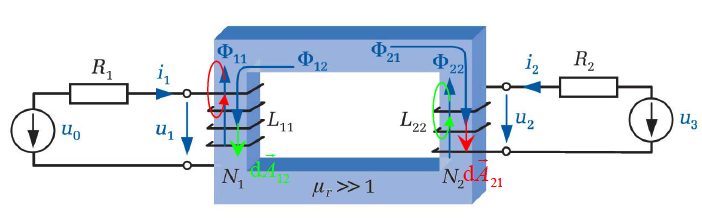
\includegraphics[width=0.75\textwidth]{img/Tra2}
\vspace{-0.2cm}
\end{figure}
Ein Transformator besteht aus (mindestens) zwei Wicklungen, die auf einem hochpermeablen Kern gewickelt und somit magnetisch eng gekoppelt sind (man kann idealerweise von einem streuungsfreien übertrager ausgehen). \newline

Wie bei der Gegeninduktion fomulieren wir die Induktivitäten aus:
$$ L_{11} = \frac{\color{red}\Phi_{11}}{i_1}, \qquad L_{22}= \frac{\color{green}\Phi_{22}}{i_2}, \qquad
M = \frac{\color{red}\Phi_{21}}{i_1}=\frac{\color{green}\Phi_{12}}{i_2}$$
(Die roten Grössen stehen für den von der linken Seite (Primärseite) erzeugten Fluss, die grünen für den von der rechten Seite (Sekundärseite) erzeugten.) Das Induktionsgesetz sagt:
 \begin{equation*}
\begin{alignedat}{2}
u_0 &= R_1i_1 + u_1 &&= R_1i_1 \color{red} + L_{11}\frac{di_1}{dt} \color{green} - M\frac{di_2}{dt} \\
u_3 &= R_2i_2 + u_2 &&= R_2i_2 \color{green} + L_{22}\frac{di_2}{dt} \color{red}-M\frac{di_1}{dt}\\
\end{alignedat}
\end{equation*}
Die negativen Vorzeichen kommen daher, dass hier bei der gewählten Zählrichtung die Sekundärflüsse $\Phi_{12},\Phi_{21}$ den Primärflüssen $\Phi_{11},\Phi_{22}$ entgegengesetzt sind. \newline


Im Fall eines streuungsfreien übertragers (aller Fluss bleibt im Magnetkern) gilt für die Induktivitäten:
$$ L_{11}= N_1^2\frac{\mu A}{l}, \qquad L_{22}= N_2^2\frac{\mu A}{l}, \qquad M = N_1N_2 \frac{\mu A}{l}$$
Und die Verhältnisse der Spannungen direkt am Transformator sind
$$u_2 =-\frac{N_2}{N_1}u_1$$
Nun betrachten wir den Fall, wo $u_3=0$:
\begin{figure}[H]
\center
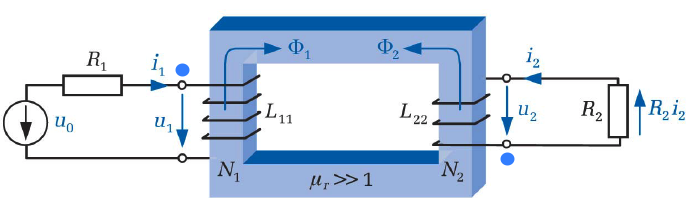
\includegraphics[width=0.75\textwidth]{img/Tra3}
\vspace{-0.2cm}
\end{figure}
In dem Fall können wir unsere Spannungsgleichungen auch schreiben als
 \begin{equation*}
\begin{alignedat}{2}
u_0 &= R_1i_1 + L_{11}\frac{di_1}{dt} - M\frac{di_2}{dt} &&= R_1i_1 + \big(L_{11}-M\big)\frac{di_1}{dt} - M \frac{d\big(i_2-i_1\big)}{dt}\\
0 &= R_2i_2 + L_{22}\frac{di_2}{dt} - M\frac{di_1}{dt} && = R_2i_2 - M \frac{d\big(i_1-i_2\big)}{dt} + \big(L_{22}-M\big) \frac{di_2}{dt} \\
\end{alignedat}
\end{equation*}
Aber das entspricht ja genau folgendem Ersatzschaltbild (das \textit{kein} physikalisch realisierbares Netzwerk darstellen muss, weil die eingezeichneten Induktivitäten ggf. negative Werte annehmen können):
\begin{figure}[H]
\center
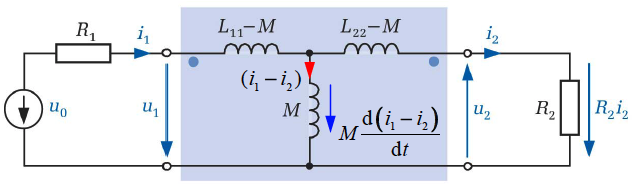
\includegraphics[width=0.75\textwidth]{img/Tra4}
\vspace{-0.2cm}
\end{figure}
Zur Punktkonvention: \newline
Die Punkte sollen den Wicklungssinn im ESB verdeutlichen, der sonst nicht ersichtlich wäre.
Auf der Primärseite kann der Punkt noch frei gewählt werden, auf der Sekundärseite muss er dann so sein, dass die Potentialdifferenz zwischen dem Wicklungsanschluss mit Punkt und dem ohne Punkt gleichzeitig positiv bzw. negativ ist wie auf der Primärseite. \newline
In der dreidimensionalen Anordnung überlegt man sich die Punkte mit der Lenz'schen Regel: $i_1$ verursacht den rechtswendig zugeordneten Fluss $\Phi_1$. Dann ist der induzierte Strom $i_2$ so gerichtet, dass sein rechtswendig zugeordneter Fluss $\Phi_2$ dem ersten Fluss $\Phi_1$ entgegenwirkt. Aus der Richtung von $i_2$ folgt über $u_2 = R_2 i_2$ die Richtung von $u_2$.\newline

\subsection{Der ideale Übertrager}
Wir haben oben schon gesehen, dass im streufreien Übertrager $$\frac{u_1}{u_2} = -\frac{N_1}{N_2} \eqdef -"u$$ gilt. Das Spannungsverhältnis von $u_1$ und $u_2$ entspricht also dem Übersetzungsverhältnis von $N_1$ und $N_2$ (Vorzeichen hängt von Zähl- und Wicklungsrichtungen ab). Wenn jetzt ausserdem noch die Permeabilität des Magneten gegen unendlich geht ($\mu_r \rightarrow \infty$), dann sprechen wir vom idealen Übertrager, und aus dem Durchflutungsgesetz folgt: $$\frac{i_1}{i_2}=\frac{N_2}{N_1} = \frac{1}{"u}$$
Das Stromverhältnis von $i_1$ und $i_2$ entspricht also gerade dem Kehrwert des Wicklungsverhältnisses (Vorzeichen wieder abhängig von Zähl- und Wicklungsrichtung). \newline

Daraus folgt auch, dass die links abgegebene Leistung $p_1$ gerade der rechtsseitig aufgenommenen Leistung $p_2$ entspricht, was intuitiv sofort Sinn macht:
$$p_1 = u_1i_1 = -"u u_2~\frac{i_2}{"u} = -u_2 i_2 = p_2$$
Ab jetzt schreiben wir für primärseitige Grössen den Index $p$ statt $1$ und für sekundärseitige Grössen $s$ statt $2$. Für den idealen Übertrager führen wir folgendes Schaltbild ein:
\begin{figure}[H]
\center
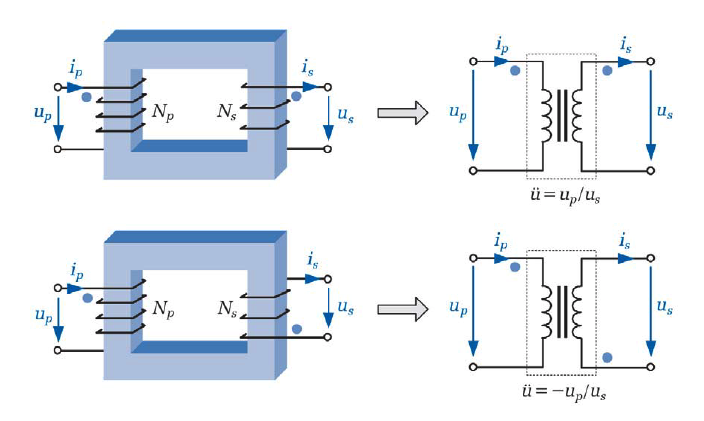
\includegraphics[width=0.75\textwidth]{img/Tra5}
\vspace{-0.2cm}
\end{figure}
Wir haben nochmal zusammengefasst:
$$"u = \frac{N_p}{N_s},\qquad \frac{u_p}{u_s} = \frac{i_s}{i_p} = \pm"u, \qquad p_p=u_pi_p=u_si_s=p_s$$
Wir betrachten nochmal die frühere Anordnung, aber in der neuen Notation:
\begin{figure}[H]
\center
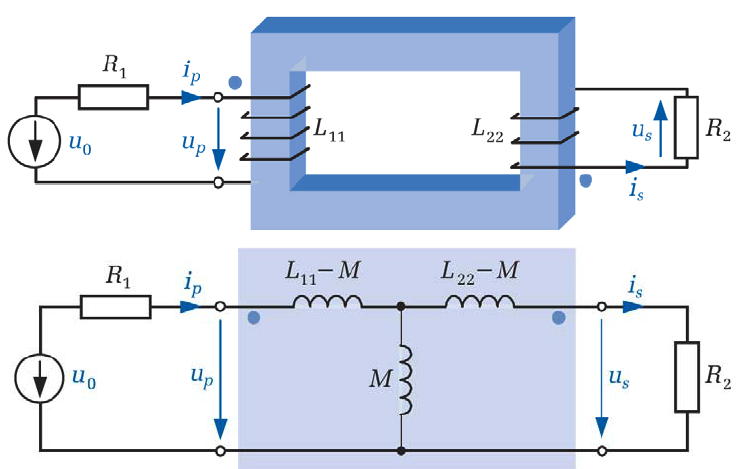
\includegraphics[width=0.65\textwidth]{img/Tra6}
\vspace{-0.2cm}
\end{figure}
Um die galvanische Trennung zwischen Ein- und Ausgangsseite zu verdeutlichen, führen wir einfach einen idealen Übertrager mit Übersetzungsverhältnis $"u=1$ ein. Das hat auf das Verhalten des Netzwerks keinen Einfluss:
\begin{figure}[H]
\center
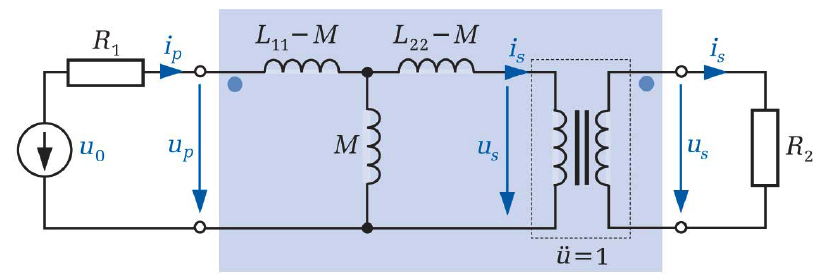
\includegraphics[width=0.65\textwidth]{img/Tra7}
\vspace{-0.2cm}
\end{figure}
Wie müssen wir aber jetzt das ESB anpassen, wenn wir ein Übersetzungsverhältnis $"u \neq 1$ haben möchten? So:
\begin{figure}[H]
\center
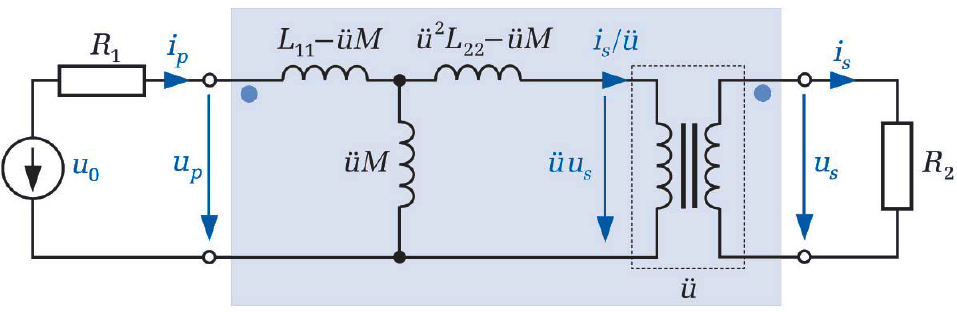
\includegraphics[width=0.65\textwidth]{img/Tra8}
\vspace{-0.2cm}
\end{figure}
Falls nun unser Transformator nicht ideal ist, können wir dem durch hinzufügen von parasitären Widerständen, welche die Verluste repräsentieren, Rechnung tragen:
\begin{figure}[H]
\center
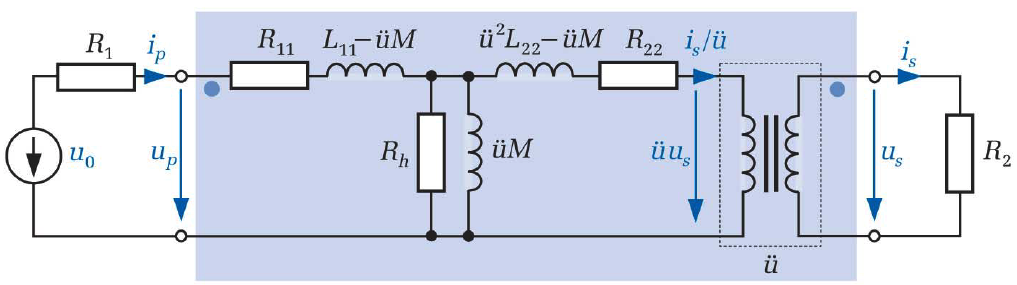
\includegraphics[width=0.75\textwidth]{img/Tra9}
\vspace{-0.2cm}
\end{figure}

\textbf{Widerstandstransformation}\newline
Wie sieht ein Widerstand auf der Sekundärseite eines idealen Übertragers von der Primärseite betrachtet aus?
\begin{figure}[H]
\center
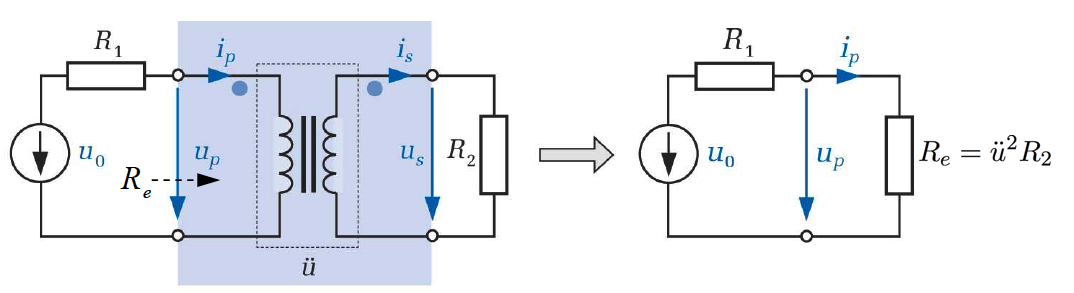
\includegraphics[width=0.85\textwidth]{img/Tra10}
\vspace{-0.2cm}
\end{figure}
Es ist
$$R_e = \frac{u_p}{i_p} = \frac{"u u_s}{\frac{i_s}{"u}}="u^2\frac{u_s}{i_s} = "u^2R_2$$
\pagebreak
